\documentclass[10pt]{article}
\setlength{\oddsidemargin}{.5in}
\setlength{\evensidemargin}{.5in}
\setlength{\textwidth}{6.0in}
\setlength{\topmargin}{0.0in}
\addtolength{\topmargin}{-1.0in}
\setlength{\footskip}{.5in}
\setlength{\textheight}{9.5in}
\linespread{1.1}

% Michael Carlisle, Baruch College, CUNY, MTH 2610, Fall 2016
% github.com/mcarlisle/lecture-notes (posted Jan 2019)

\usepackage{graphicx}
\usepackage{epsfig}
\usepackage{amssymb}
\usepackage{amsmath}


\begin{document}

\pagenumbering{gobble}

%---:----1----:----2----:----3----:----4----:----5----:----6----:----7----:---

\begin{center}
Calculus I Quiz \#5
\end{center}



\noindent\textbf{Problem 1} \,\, We wish to fence in a rectangular area of 10,000 square meters against a river with a straight-line coast. What dimensions are needed for the least amount of fencing if no fencing is needed along the river?

\begin{figure}[!ht]
    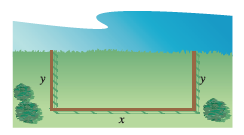
\includegraphics[width=2in]{fencing.png}
\end{figure}

\vspace{70mm}

\noindent\textbf{Problem 2} \,\, For the cost function $C(x) = 2x^2 + 5x + 18$, where $x$ is the number of items produced, find the minimum average cost, and show that the marginal cost equals the average cost at that level of production. 
% unless you're making pizzas, quadratic cost functions are ridiculous

\end{document}
